\section{Clustering}

Il metodo di identificazione di dispositivi ignoti a partire da un'insieme di immagini digitali campioni prevede una fase di clustering che, usando la PNRU di ciascuna immagine, va a suddividere tale insieme in un sotto insieme di immagini simili, ovvero con lo stesso pattern noise e quindi, presumibilmente, provenienti dallo stesso sensore.
L'insieme delle PNRU delle immagini viene rappresentato con un grafo pesato completamente connesso, in cui le PNRU, e quindi le immagini, rappresentano i nodi. I pesi associati a ciascun arco sono calcolati con la PCE (Peak-to-Correlation Energy), una misura di similarità che si adatta molto bene per le fingerprint, calcolate con la PNRU, di immagini bidimensionali. La caratteristica principale di tale misura è che la presenza di patter periodici nascosti diminuisce la PCE. Quindi il peso associato all'arco sarà tanto più alto quanto i nodi interessati avranno una PNRU simile. Il grafo pesato può essere rappresentato da una matrice quadrata $NxN$, con N numero di immagini.
Calcolare la PCE per tutti i nodi del grafo è una delle operazioni più costose del metodo di identificazione implementato, infatti calcolare la matrice dei pesi ha complessità quadratica con il numero di immagini.

Una volta costruito il grafo pesato possiamo procedere con la fase di clusterizzazione, per suddividere le immagini in gruppi di immagini simili, in base alla loro PNRU.


\subsection{Normalized Cuts}

Dato una grafo $ G = <V, E> $, gli archi $E$ che connettono ciascuna coppia di nodi, ovvero di PNRU, sono pesati con la PCE, come descritto in precedenza, dove $PCE(i, j)$ rappresenta la similarità fra il nodo $i$ e il nodo $j$.
L'algoritmo di clusterizzazione Normalized Cuts è un algoritmo ricorsivo, che ad ogni iterazione, bipartiziona il grafo G, creando quindi due sottografi A e B ($A\cup B = V$ e $A\cap B = \emptyset$). Una volta ottenuti due sottografi è possibile dare un valore del taglio ovvero calcolare il peso totale  degli archi rimossi che fornisce una stima sul grado di dissimilarità di questi due sottografi. Il taglio è calcolato come segue: $$ cut(A,B) = \sum_{u\in A, v\in B} w(u, v) $$

Il taglio ottimale per bipartizionare il grafo è calcolato ottimizzando il valore di un taglio normalizzato taglio, ideato dagli autori originali dell'algoritmo per evitare che si favorisca la creazione di piccoli cluster composti da nodi isolati. Il taglio normalizzato, da cui l'algoritmo Normalized Cuts prende il nome, è calcolato come segue: 
$$ Ncut(A,B) =  \frac{cut(A,B)}{assoc(A,V)} + \frac{cut(A,B)}{assoc(B,V)} $$
dove $assoc(A,V) = \sum_{u\in A, t\in V} w(u,t) $ rappresenta la somma dei pesi degli archi che connettono i nodi della partizione A ad un generico nodo del grafo G.
Va notato che la misura di $cut(A,B)$ è sempre minore di $assoc(A,V)$ e di $assoc(B,V)$. Gli archi che sono rimossi sono una frazione degli archi che hanno un nodo in A e l'altro nodo in B. Il valore $assoc(A,V) - cut(A,B)$ misura la somma dei pesi degli archi che collegano due nodi in A. Quindi, il valore di $ \frac{cut(A,B)}{assoc(A,V)}$ è basso quando i nodi in A hanno un grado di similarità fra di loro ad un basso grado di similarità con in nodi che non appartengono i A. Il taglio normalizzato ha quindi la proprietà di partizionare il grafo in due segmenti A e B tale che la somma dei pesi degli archi che connettono le due partizioni è bassa.

Per calcolare il taglio normalizzato ottimale, occorre:
\begin{itemize}
\item una matrice dei pesi, calcolata nel nostro caso con la PCE, che rappresenta la similarità fra ciascun nodo.
\item un vettore di componenti $\gamma$, che rappresenta il taglio, di dimensione pari al numero di nodi del grafo. Il valore dell'i-esimo componente è pari a 1 se l'i-esimo nodo appartiene al primo segmento; è pari a 0 se l'i-esimo nodo appartiene alla seconda partizione.
\item una degree matrix $D = \lbrace d_{ii} \rbrace $, una matrice diagonale, in cui ogni elemento è sulla diagonale è la somma di tutti i pesi degli archi che partono dall'i-esimo nodo, ovvero $d_{ii} = \sum_{j} a_{ij}$
\end{itemize}

Può essere dimostrato che il taglio che minimizza il costo normalizzato, minimizza anche la seguente funzione: $$ \frac{\gamma^{T}(D-A)\gamma}{\gamma^{T}D\gamma}$$
La soluzione $\gamma$, che rappresenta il taglio, dovrebbe essere un vettore di valori discreti in $\lbrace 0,1 \rbrace$. Tale funzionale è una versione discreta del quoziente di Rayleigh. Risolve tale funzionale per valori discreti è un problema NP-completo. Tuttavia, il problema diventa trattabile se la soluzione $\gamma$ è libera di assumere valori reali. A questo punto, minimizzare il costo di una funzione per un vettore $\gamma$ di valori reali è equivalente alla soluzione della seguente equazione: $$ (D-A) \gamma = \lambda D \gamma $$
Poichè il più piccolo autovalore di $(D-A)$ è pari a zero, può essere dimostrato che la soluzione all'equazione è l'autovettore corrispondente al secondo più piccolo autovalore.
Una volta ottenuto la soluzione reale è necessario discretizzarla nei valori $\lbrace 0,1 \rbrace$. Per fare ciò occorre scegliere un valore di soglia. Per fare ciò si può utilizzare il valore 0 o il valore mediano fra gli elementi della soluzione come valore di soglia oppure si può scegliere il valore, fra gli elementi della soluzione, che minimizza il valore di $Ncut(A,B)$.

La procedura di bipartizione del grafo può essere riassunta come segue:
\begin{enumerate}
\item Dato un insieme di features, costruire un grafo pesato $G = <V,E>$, calcolando i pesi di ciascun arco che rappresentano una similarità fra i nodi.
\item Risolvere l'equazione mostrata precedentemente Eq.(num) utilizzando l'autovettore corrispondente al secondo più piccolo autovalore.
\item Usare tale soluzione per bipartizionare il grafo, in modo tale che il costo del taglio normalizzato sia minimo.
\item Decidere se le due partizione correnti devono essere suddivise ricorsivamente andando a calcolare una misura della stabilità del taglio.
\end{enumerate}

Nella seguente sottosezione verrà spiegato in maggiore dettaglio lo step 4.

\subsubsection{Soglie}

L'algoritmo Normalized Cuts si basa su uno step ricorsivo che dipende dalla verifica di stabilità del taglio appena realizzato. L'implementazione originale dell'algoritmo prevede di comparare il valore di $Ncut(A,B)$ ad una soglia $T_{k}$ decisa a priori. Gli autori di [cit] hanno invece definito un coefficiente di aggregazione, $AC(k) = \frac{1}{N_{k}} \sum_{i,j} w(i,j)$, ovvero il valore medio dei pesi associati ai nodi che appartengono alla partizione $k$, calcolato per ciascuna partizione ottenuta; se tale valore è minore di una soglia $T_{k}$ predefinita la partizione viene ulteriormente suddivisa, se è maggiore l'iterazione si ferma.

Per decidere quali dei due metodi usare nella nostra implementazione e quale soglia $T_{k}$ predefinita utilizzare, è stato usato un approccio basato su curve ROC prendendo come parametri di correttazza della clusterizzazione il valori di TPR e FPR rispetto ad un ground-truth. Per fare ciò abbiamo considerato un sottoinsieme di 20 immagini da ciascun dispositivo del dataset utilizzato, in modo da considerare tutte i dispositivi in nostro possesso per la scelta della soglia $T_{k}$.

Il range di variazione della soglia $T_{k}$ differisce a seconda del metodo utilizzato, ovvero il valore di $Ncut$ o il coefficiente di aggregazione. I grafici mostrati in seguito rappresentano l'andamento dei valori di TPR e FPR al variare della soglia. Tali esperimenti sono stati fatti sia per le immagini direttamente acquisite dai dispositivi, sia per le immagini caricate e riscaricate da facebook, con l'opzione per il download ad alta risoluzione.

\begin{figure}[h]
\begin{center}
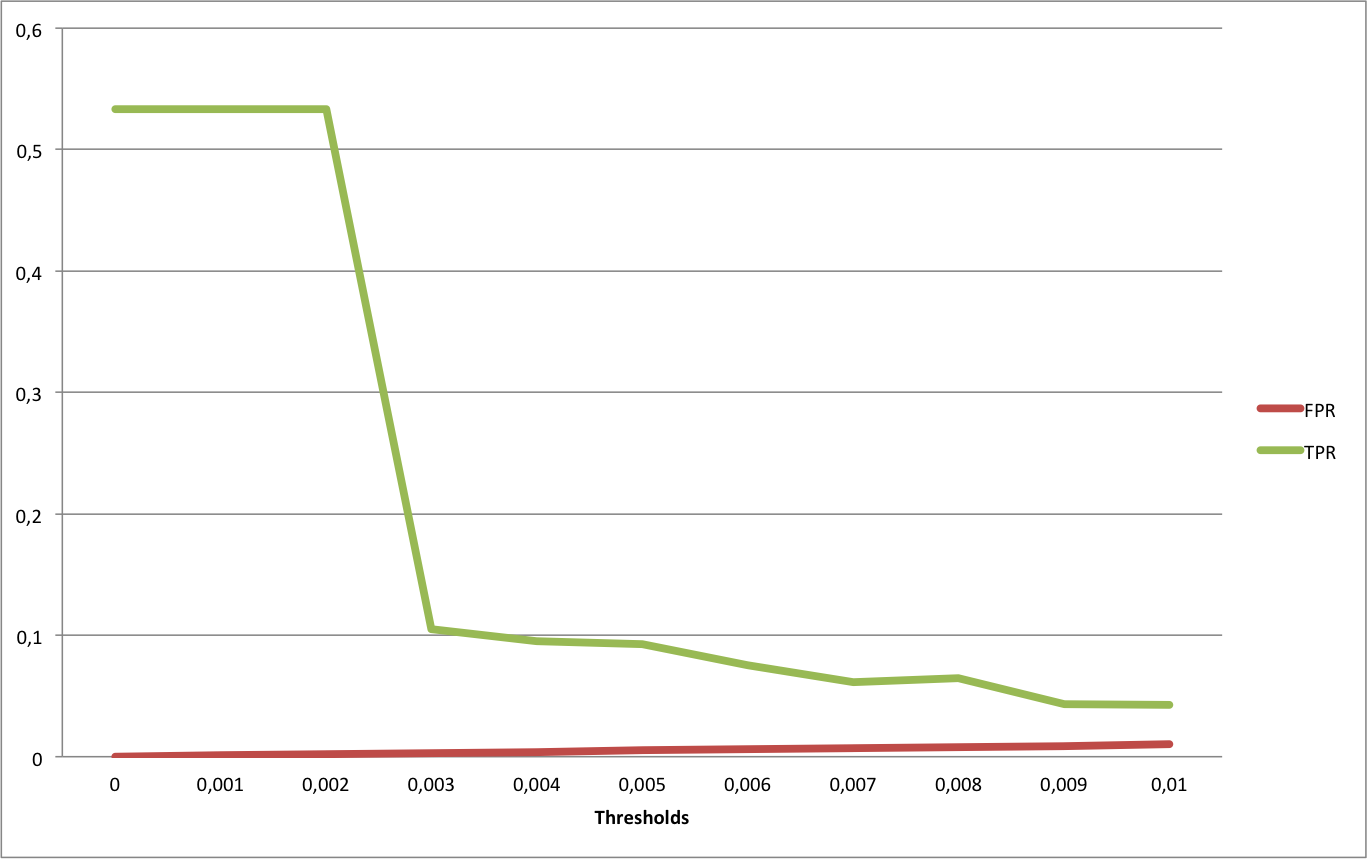
\includegraphics[width=0.4\textwidth]{images/soglia_imgnat_AC.png}
\end{center}
  \caption{Valori di TPR e FPR al variare della soglia per le immagini naturali acquisite direttamente dai dispositivi. Metodo con coefficiente di aggregazione.}
\label{fig:soglia AC}
\end{figure}

\begin{figure}[h]
\begin{center}
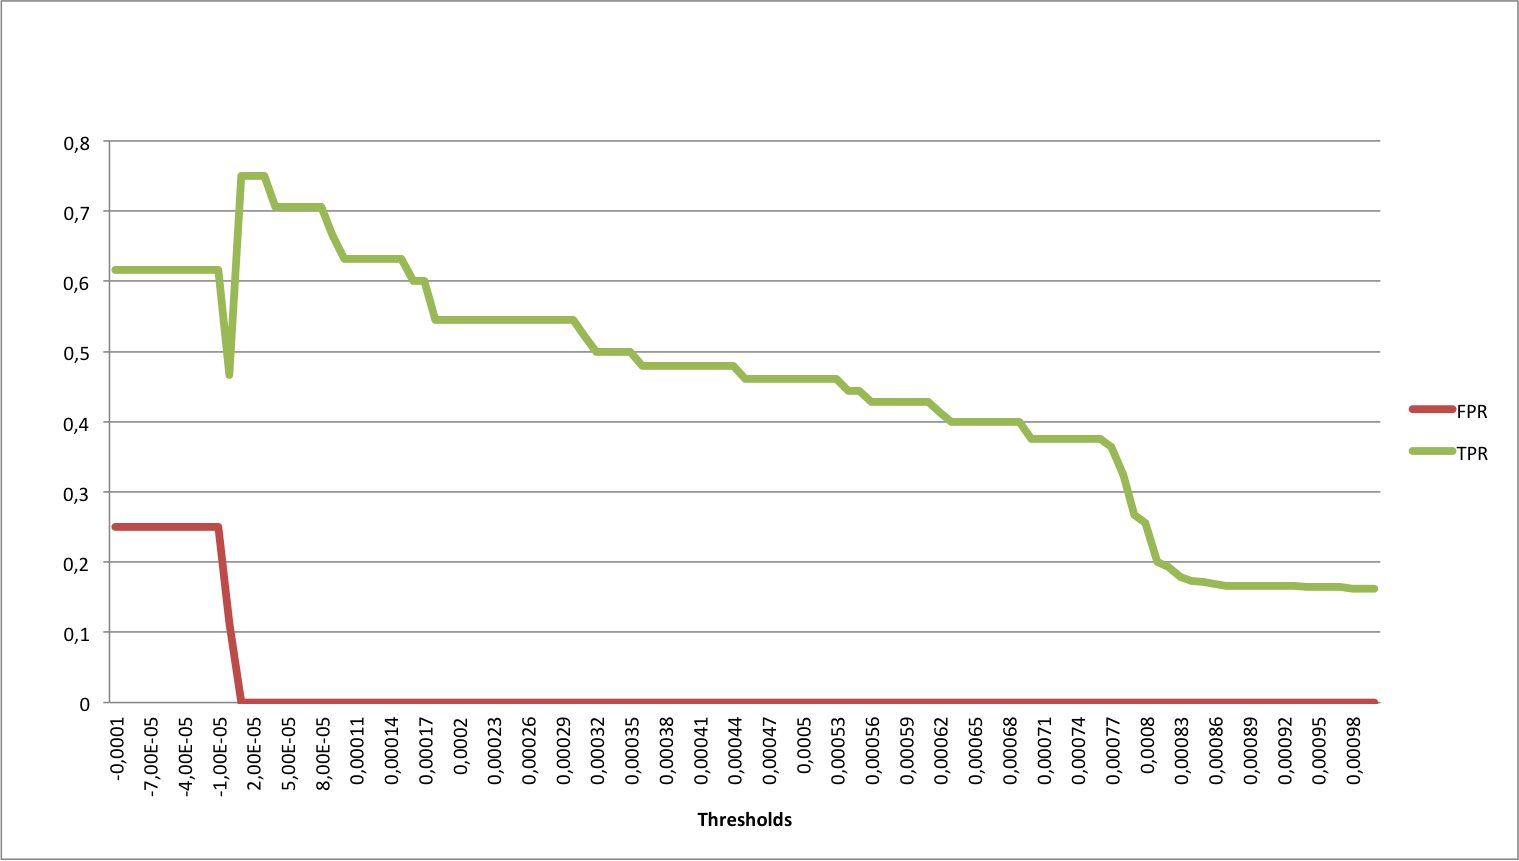
\includegraphics[width=0.4\textwidth]{images/soglia_imgnat_NC.png}
\end{center}
  \caption{Valori di TPR e FPR al variare della soglia per le immagini naturali acquisite direttamente dai dispositivi. Metodo che considera i valori di $Ncuts$.}
\label{fig:soglia AC}
\end{figure}

\begin{figure}[h]
\begin{center}
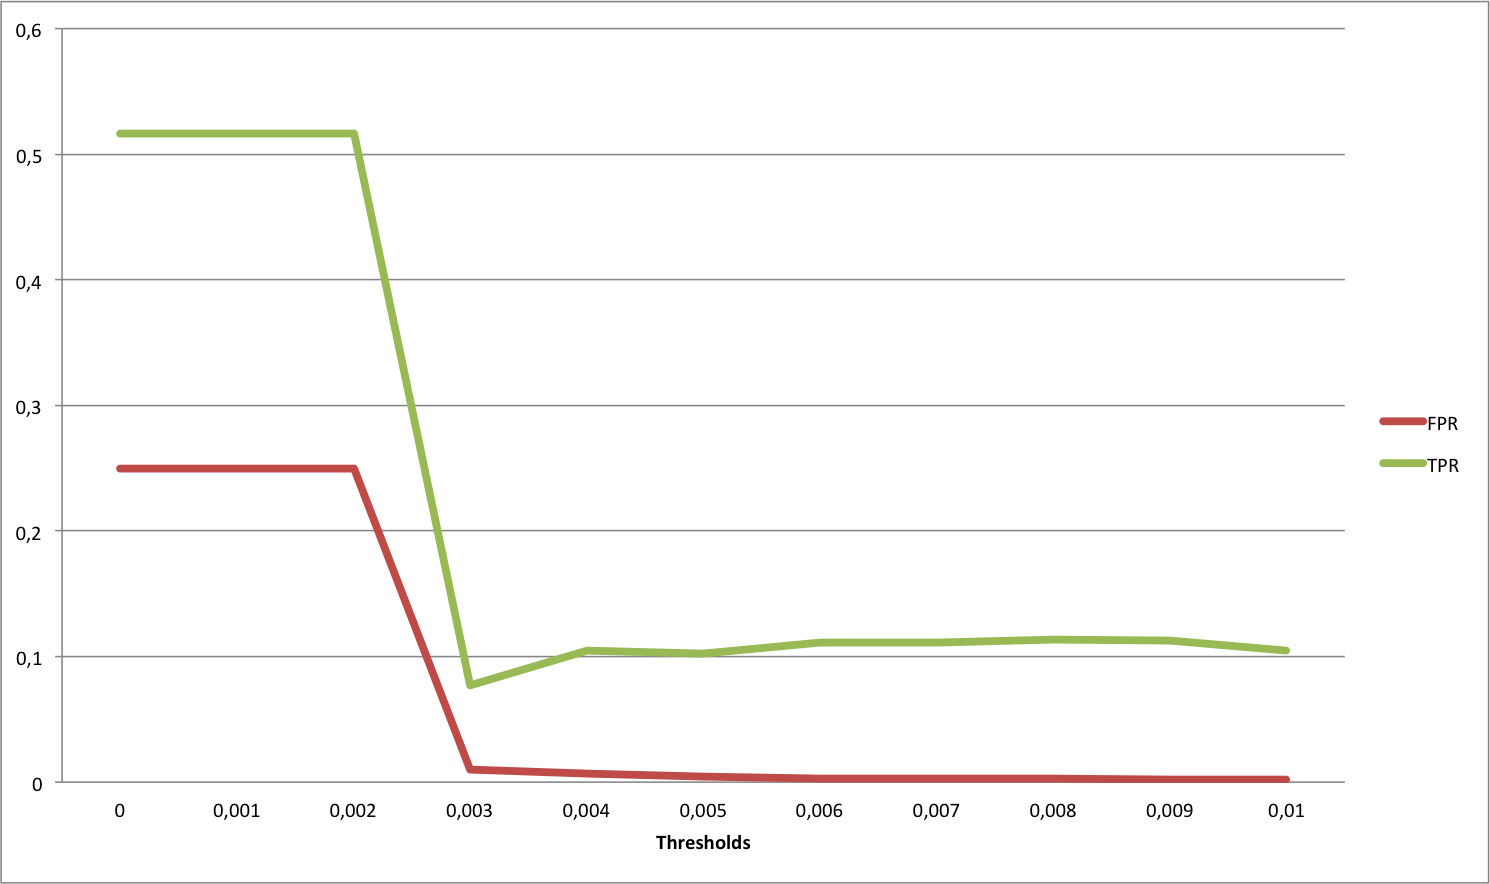
\includegraphics[width=0.4\textwidth]{images/soglia_imgnat_fb_AC.png}
\end{center}
  \caption{Valori di TPR e FPR al variare della soglia per le immagini scaricate da Facebook. Metodo con coefficiente di aggregazione.}
\label{fig:soglia AC}
\end{figure}

\begin{figure}[h]
\begin{center}
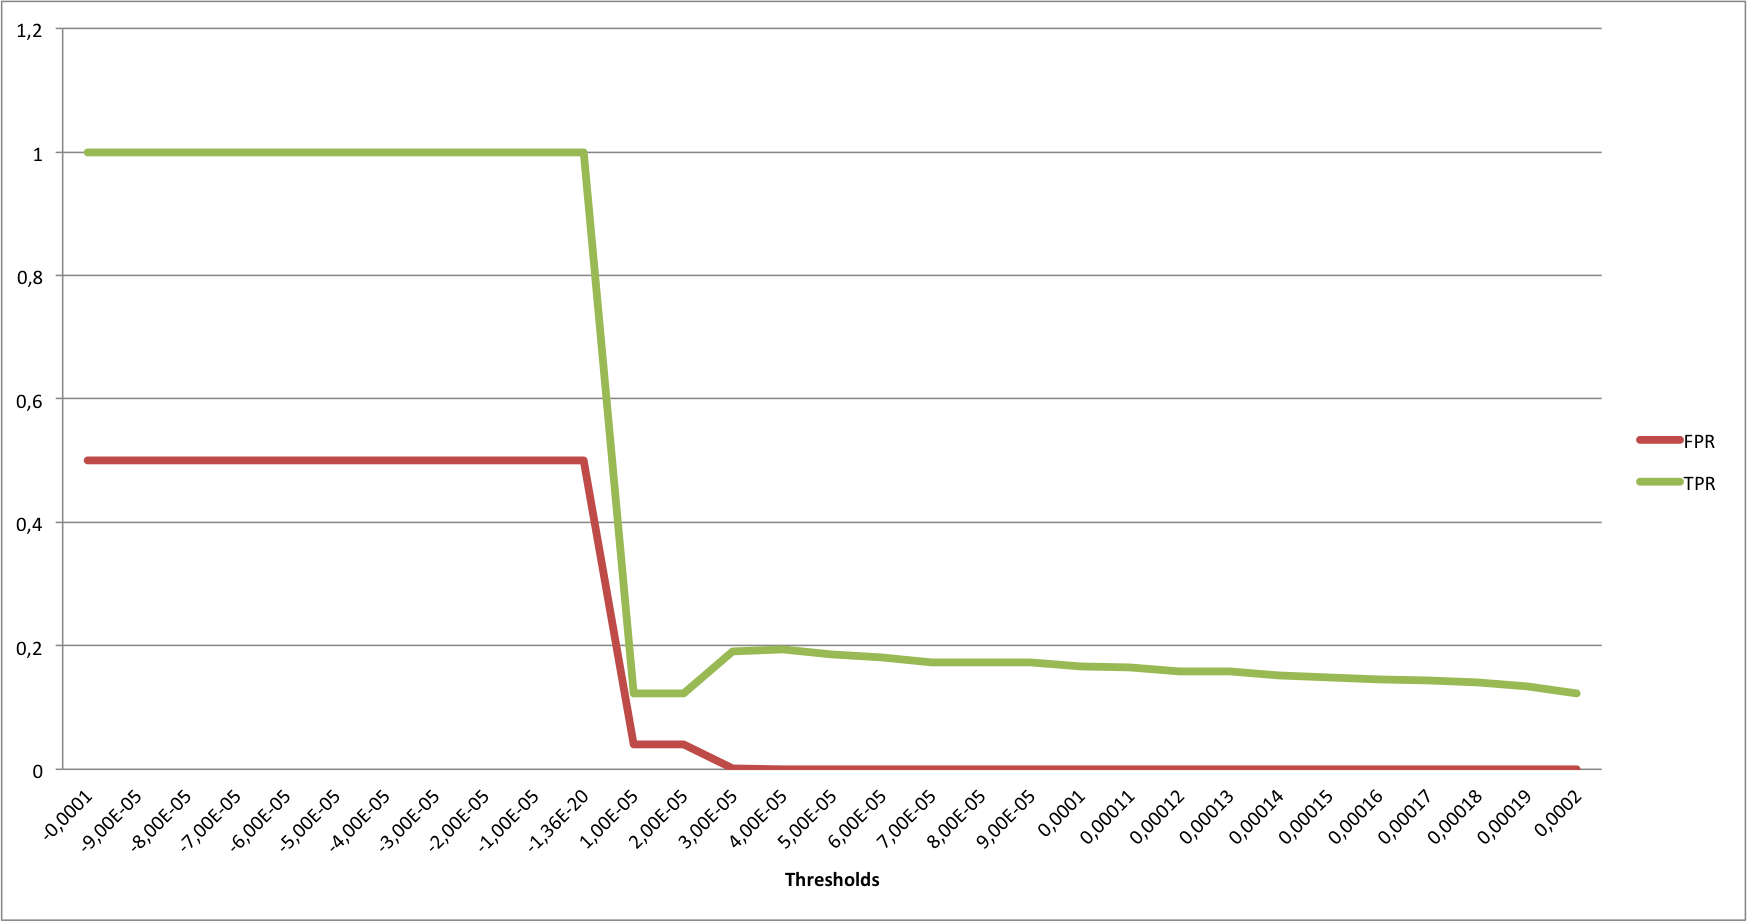
\includegraphics[width=0.4\textwidth]{images/soglia_imgnat_fb_NC.png}
\end{center}
  \caption{Valori di TPR e FPR al variare della soglia per le immagini scaricate da Facebook. Metodo che considera i valori di $Ncuts$.}
\label{fig:soglia AC}
\end{figure}

Nella nostra implementazione, come si può notare dai risultati, il metodo che utilizza $Ncut$ risulta essere il migliore quando vengono usate le immagini direttamente acquisite dai dispositivi. Per questo caso è stata selezionata come migliore soglia $T_{k} = 10^{-5}$ che corrisponde al valore massimo di TPR, pari a 0.75, e al valore minimo di FPR, pari a 0; ciò significa che le immagini non sono perfettamente raggruppate, ovvero il numero di clusters è maggiore di quello atteso, ma al contempo i clusters ottenuti sono "puliti" ovvero sono composti solo da elementi simili, non contengono,cioè, falsi positivi.
Per il caso delle immagini provenienti da Facebook, il confronto fra i due metodi è più incerto. Ciò è probabilmente dovuto al fatto che, subendo una compressione, la PNRU di tali immagini perde informazione in grado di discriminarle a sufficienza. Infatti i risultati ottenuti mostrano un numero significativo di falsi positivi contenuti nei clusters in entrambi i metodi, una situazione non desiderabile poichè è a partire da tali clusters che verranno calcolate le fingerprint relative ai dispositivi. Inoltre i minimi valori di FPR si ottengono in corrispondenza dei minimi valori di TPR; ciò indica che i clusters ottenuti sono perlopiù cluster singoli o con pochi elementi, altro caso non desiderabile. Tuttavia, per coerenza con il caso precendete, è stata scelto di utilizzare il metodo relativo a $Ncuts$, poichè mostra più consistenza con il valore ottimale della soglia $T_{k}$, che è sempre pari a $10^{-5}$ e che corrisponde al valore minimo di FPR.

In generale la scelta della soglia ottimale è stata fatta minimizzando il valore dei falsi positivi all'interno dei clusters calcolati; è preferibile ottenere più clusters ma che genereranno fingerprint senza rumore, piuttosto che un numero esatto di clusters da cui però si otterranno fingerprint rumorose.
